\documentclass{standalone}
\usepackage{tikz}
\usetikzlibrary{automata, positioning}

\begin{document}
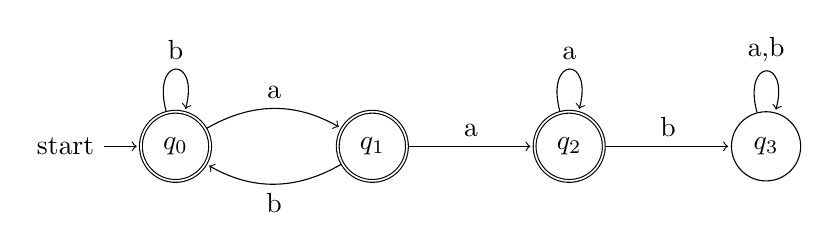
\begin{tikzpicture}[shorten >=1pt, node distance=2.5cm, on grid, auto]
  \node[state, initial, accepting] (q_0) {$q_0$};
  \node[state, accepting] (q_1) [right=of q_0] {$q_1$};
  \node[state, accepting] (q_2) [right=of q_1] {$q_2$};
  \node[state] (q_3) [right=of q_2] {$q_3$};
  \path[->]
    (q_0) edge[bend left] node {a} (q_1)
    (q_0) edge[loop above] node {b} ()
    (q_1) edge[bend left] node {b} (q_0)
    (q_1) edge node {a} (q_2)
    (q_2) edge[loop above] node {a} ()
    (q_2) edge node {b} (q_3)
    (q_3) edge[loop above] node {a,b} ()
    ;
\end{tikzpicture}
\end{document}